%%%%%%%%%%%%%%%%%%%%%%%%%%%%%%%%%%%%%%%%%
% University/School Laboratory Report
% LaTeX Template
% Version 3.1 (25/3/14)
%
% This template has been downloaded from:
% http://www.LaTeXTemplates.com
%
% Original author:
% Linux and Unix Users Group at Virginia Tech Wiki 
% (https://vtluug.org/wiki/Example_LaTeX_chem_lab_report)
%
% License:
% CC BY-NC-SA 3.0 (http://creativecommons.org/licenses/by-nc-sa/3.0/)
%
%%%%%%%%%%%%%%%%%%%%%%%%%%%%%%%%%%%%%%%%%

%----------------------------------------------------------------------------------------
%	PACKAGES AND DOCUMENT CONFIGURATIONS
%----------------------------------------------------------------------------------------
\PassOptionsToPackage{table}{xcolor}

\documentclass[a4paper,twoside]{article}

\usepackage[a4paper,margin=1in]{geometry}
\usepackage[english]{babel}
\usepackage{fancyhdr}
\usepackage{titling}
\usepackage{lastpage}
\usepackage{subcaption}
\usepackage{graphicx}
\usepackage{enumitem}
\usepackage[toc,page]{appendix}

\usepackage[style=ieee, backend=biber]{biblatex}
\addbibresource{biblio.bib}

\usepackage{forloop}% http://ctan.org/pkg/forloop
\newcounter{loopcntr}
\newcommand{\rpt}[2][1]{%
	\forloop{loopcntr}{0}{\value{loopcntr}<#1}{#2}%
}

\usepackage[separate-uncertainty=true]{siunitx}
\DeclareSIUnit\sq{\ensuremath{\Box}}
\DeclareSIUnit\photon{ph}
\DeclareSIUnit\dec{dec}
\DeclareSIUnit\electron{e^-}
\DeclareSIUnit\LSB{LSB}
\DeclareSIUnit\rms{rms}
\sisetup{detect-weight=true,range-phrase = \text{--}}

\usepackage{hyperref}%
\usepackage{pdfpages}
\usepackage{booktabs}
\usepackage{multirow}
\usepackage{csvsimple}
\def\localpath{D:/Documents/PhD/FALCON/tex/data/}
\captionsetup[table]{position=bottom,skip=3pt}

\usepackage[siunitx, RPvoltages, arrowmos]{circuitikz}
\usepackage{tikz}
\usetikzlibrary{shapes,arrows,positioning,calc,automata}
\tikzset{
	->, % makes the edges directed
	>=stealth, % makes the arrow heads bold
	node distance=3.5cm, % specifies the minimum distance between two nodes. Change if necessary.
	every state/.style={thick, fill=gray!10}, % sets the properties for each ’state’ node
	initial text=$ $, % sets the text that appears on the start arrow
}
% circuitikz
\ctikzset{tripoles/pmos style/nocircle}

\usepackage{pgfplots}
\usetikzlibrary{pgfplots.groupplots}

\usepackage[nottoc]{tocbibind}


\usepackage[nottoc]{tocbibind}

\usepackage{amsmath, mathtools, amssymb}
\DeclareMathOperator*{\argmax}{arg\,max}
\DeclareMathOperator*{\argmin}{arg\,min}
\DeclareMathOperator\erf{erf}

\makeatletter
\newcommand*{\textoverline}[1]{$\overline{\hbox{#1}}\m@th$}
\makeatother

\usepackage{bytefield}
\usepackage[outline]{contour}
\usepackage{afterpage}

%\usepackage{setspace}
%\onehalfspacing

\usepackage{url}
\renewcommand{\UrlFont}{\small}

%\setlength\parindent{0pt} % Removes all indentation from paragraphs

\renewcommand{\labelenumi}{\arabic{enumi}.} % Make numbering in the enumerate environment by number and not letter

% remove table of contents title
\makeatletter
\renewcommand\tableofcontents{%
	\@starttoc{toc}%
}
\makeatother

%\usepackage{times} % Uncomment to use the Times New Roman font

\pagestyle{fancy}
\fancyhf{}
\fancyhead[LE,RO]{Activities of the second Ph.D. year}
\fancyhead[RE,LO]{\leftmark}
\fancyfoot[LE,RO]{P. Lazzaroni}
\fancyfoot[CE,CO]{Page \thepage\ of \pageref{LastPage}}
\fancyfoot[RE,LO]{\today}

\fancypagestyle{first}{%
	\fancyhf{}
	\renewcommand{\headrulewidth}{0pt}%
	\lfoot{P. Lazzaroni}
	\cfoot{Page \thepage\ of \pageref{LastPage}}
	\rfoot{\today}
}

%\usepackage{times} % Uncomment to use the Times New Roman font

%----------------------------------------------------------------------------------------
%	DOCUMENT INFORMATION
%----------------------------------------------------------------------------------------

\title{\fontsize{22}{18}\selectfont \textbf{pFREYA DAQ documentation}}
\author{\fontsize{16}{18}\selectfont Paolo \textsc{Lazzaroni}\\{\textmu}Lab\\Università degli Studi di Bergamo}

\begin{document}
	
	\maketitle\thispagestyle{empty} % Insert the title, author and date
	
	\section*{Summary}
	
	This document provides information on the Data AQuisition (DAQ) system to test the pFREYA16 and pFREYATS ASICs. The system is based on a Xilinx Ultrascale+ FPGA Evaluation Board (KCU116) and it is written in SystemVerilog/Verilog.
	
	\tableofcontents
	\clearpage
	
	\section{State machine}
	This section illustrate the state machine on the FPGA.
	\begin{figure}[h]
		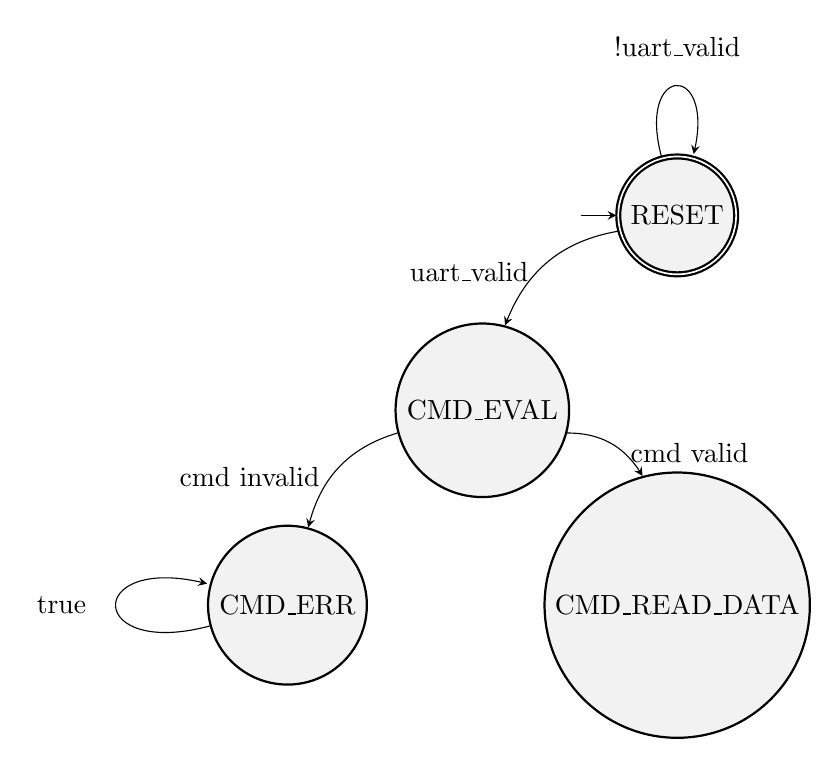
\begin{tikzpicture}
			\centering
			\node[state, initial, accepting] (RESET) {RESET};
			\node[state, below left of=RESET] (CMD_EVAL) {CMD\_EVAL};
			\node[state, below left of=CMD_EVAL] (CMD_ERR) {CMD\_ERR};
			\node[state, below right of=CMD_EVAL] (CMD_READ_DATA) {CMD\_READ\_DATA};
	
			\draw (RESET) edge[loop above] node[label=above:!uart\_valid]{} (RESET);
			\draw (RESET) edge[below, bend right] node[label=left:uart\_valid]{} (CMD_EVAL);
			\draw (CMD_EVAL) edge[below, bend left] node[label=right:cmd valid]{} (CMD_READ_DATA);
			\draw (CMD_EVAL) edge[below, bend right] node[label=left:cmd invalid]{} (CMD_ERR);
			\draw (CMD_ERR) edge[loop left] node[label=left:true]{} (CMD_ERR);
		\end{tikzpicture}
	\end{figure}

%----------------------------------------------------------------------------------------
%	BIBLIOGRAPHY
%----------------------------------------------------------------------------------------

\clearpage
\nocite{*}
\printbibliography
%----------------------------------------------------------------------------------------


\end{document}